\documentclass{article}
\usepackage{pgfplots}
\usepgfplotslibrary{smithchart}

\pgfplotsset{compat=1.12}

\begin{document}

\subsection{Smith Charts}

\begin{pgfplotslibrary}{smithchart}
	A library to draw Smith Charts.

	A Smith Chart maps the complex half plane with positive real parts to the unit circle. The |smithchart| library allows \PGFPlots\ to visualize Smith Charts: it visualizes two--dimensional input coordinates $z \in \C $ of the form $z = x+ j y \in \C$ ($j$ being the imaginary unit, $j^2=-1$) with $x \ge 0$ using the map
	\[ r\colon [0,\infty] \times [-\infty,\infty] \to \{ a+j b \;\vert\;  a^2 + b^2 = 1 \}, \quad r(z) = \frac{z-1}{z+1} \]
	using complex number division. The result is always in the unit circle.

	The main application for Smith Charts is in the area of electrical and electronics engineers specializing in radio frequency: to show the reflection coefficient $r(z)$ for normalised impedance $z$. It is beyond the scope of this manual to delve into the radio frequency techniques; for us, it is important to note that the |smithchart| library supports
	\begin{itemize}
		\item the data map $r(z)$ shown above,
		\item an axis class which interprets $x$ as the real components and $y$ as the imaginary components,
		\item a visualization of grid lines as arcs,
		\item the possibility to stop grid lines to allow uniform spacing in Smith Charts,
		\item a large set of the \PGFPlots\ axis fine tuning parameters,
		\item input of already mapped coordinates $r(z)$ (i.e.\ Cartesian coordinates in the unit circle),
		\item many of the \PGFPlots\ plot handlers.
	\end{itemize}
\end{pgfplotslibrary}

\subsubsection{Smith Chart Axes}

\begin{environment}{{smithchart}\oarg{options}}
	The |\begin{smithchart}| environment draws Smith Charts. It accepts the same \meta{options} as |\begin{axis}|. In fact, it is equivalent to |\begin{axis}[|\meta{options}|,axis type=smithchart]|.
\begin{codeexample}[]
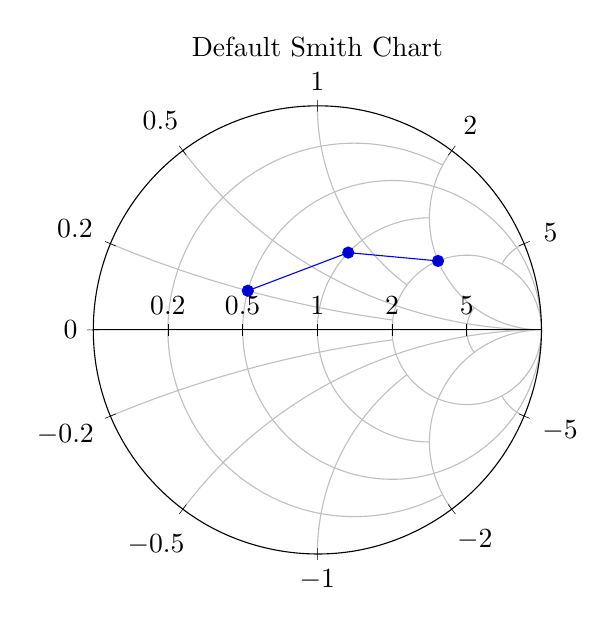
\begin{tikzpicture}
	\begin{smithchart}[title=Default Smith Chart]
	\addplot coordinates {(0.5,0.2) (1,0.8) (2,2)};
	\end{smithchart}
\end{tikzpicture}
\end{codeexample}
	The example above visualizes three data points using the initial configuration of Smith Charts; the data points are interpreted as complex numbers $z = x + j y$ and are mapped using $r(z)$.

\end{environment}

\subsubsection{Size Control}
A Smith Chart can be resized by providing either |width| or |height| as argument to the axis. If you provide both, the Chart is drawn as an ellipsis.

The tick and grid positions for |smithchart| axes are realized by means of three manually tuned sets of grid lines: one for small-sized plots, one for medium-sized plots and one for huge plots. The actual parameters for |width| or |height| are considered to select one of the following sets:

\begin{stylekey}{/pgfplots/few smithchart ticks}%
	This produces the output of the example above -- it constitutes the initial configuration for Smith Chart which has a width of less than |14cm|.
	
	The |few smithchart ticks| style is defined by:
\begin{codeexample}[code only]
\pgfplotsset{
	few smithchart ticks/.style={
		default smithchart xtick/.style={
			xtick={0.2,0.5,1,2,5},
		},
		default smithchart ytick/.style={
			ytick={%
				0,%
				 0.2, 0.5, 1, 2, 5,%
				-0.2,-0.5,-1,-2,-5},
		},
		default smithchart xytick/.style={
			xgrid each nth passes y={2},
			ygrid each nth passes x={2},
		},
	},
}
\end{codeexample}
	\noindent Note that |few smithchart ticks| contains syntactical overhead to distinguish between ``default ticks'' and final tick positions: it does not assign |xtick| and |ytick| directly. Instead, it provides them as separate |default xtick style| arguments. The purpose of this distinction is to mark them as ``default'' arguments -- the underlying styles |smithchart/every default xtick| is used if and only if there is no |xtick| value given.
	
	In case you want to override this default, you can either
	\begin{itemize}
		\item copy--paste the definition above and adjust it or
		\item omit all the |default smithchart xtick/.style| stuff and write |xtick=|\marg{your list} directly.
	\end{itemize}
	As mentioned, the only purpose of the |default smithchart xtick/.style| overhead is to distinguish between |\begin{smithchart}[xtick=|\marg{user defined}|]| and default arguments (see the documentation of |default smithchart xtick/.style| for more about this technical detail).

	
	For fine tuning of the scaling decisions, see the |smith chart ticks by size| key.

\end{stylekey}

\begin{stylekey}{/pgfplots/many smithchart ticks}%
	The |many smithchart ticks| style is used for every Smith Chart whose width exceeds |14cm| although it is less than |20cm|:
\begin{codeexample}[]
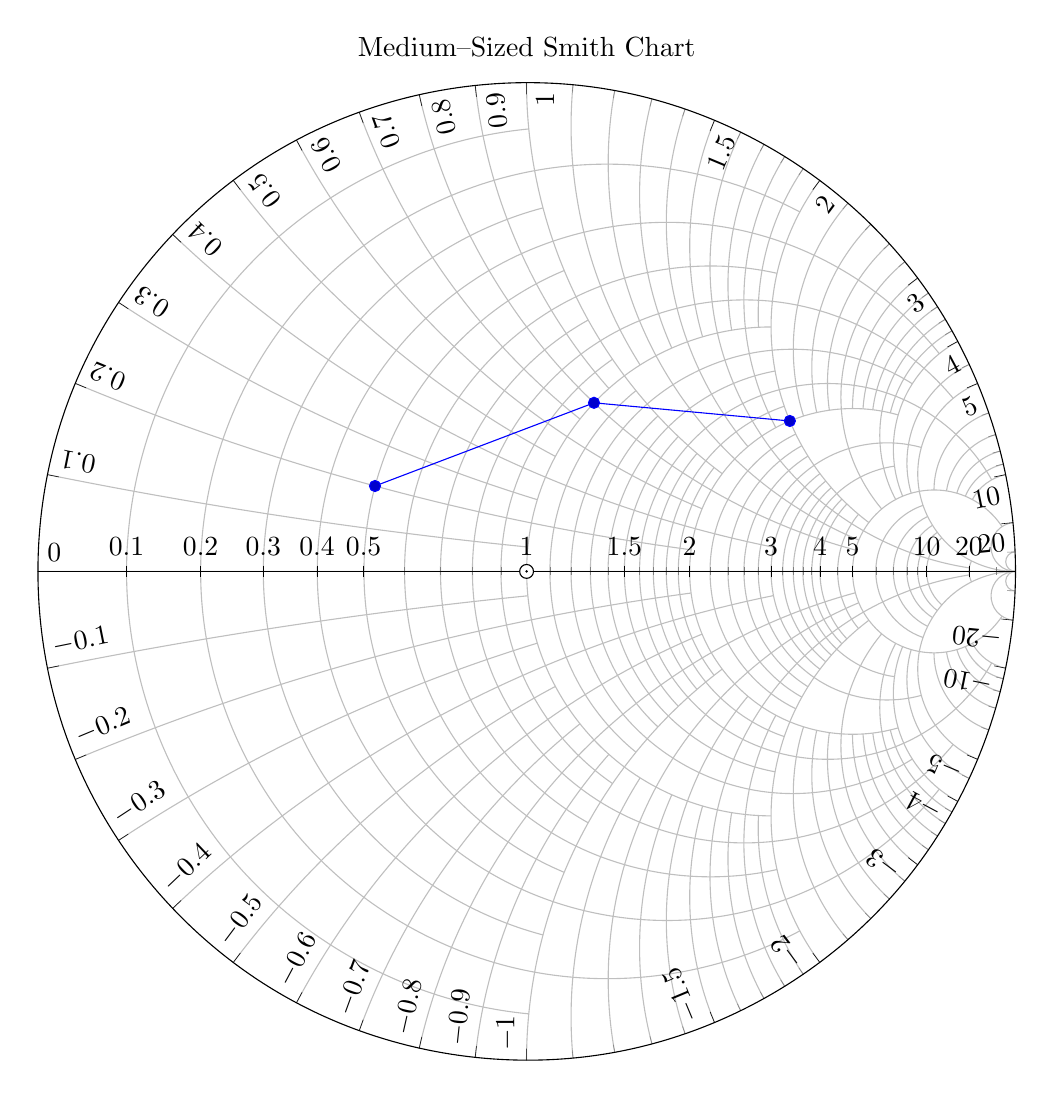
\begin{tikzpicture}
	\begin{smithchart}[
		title=Medium--Sized Smith Chart,
		width=14cm]
	\addplot coordinates {(0.5,0.2) (1,0.8) (2,2)};
	\end{smithchart}
\end{tikzpicture}
\end{codeexample}
	
	We see that |many smithchart ticks| has different placement and alignment options than |few smithchart ticks|: it uses sloped tick labels inside of the unit circle for the $y$ descriptions (imaginary axis).

	The initial configuration is realized by means of \emph{two} separate styles: one which defines only the tick positions (the \declareandlabel{many smithchart ticks*} style) and one which also changes placement and alignment options. The initial configuration can be changed individually (see the end of this section for examples). The initial configuration is:
\begin{codeexample}[code only]
\pgfplotsset{
	many smithchart ticks*/.style={
		default smithchart xtick/.style={
			xtick={
				0.1,0.2,0.3,0.4,0.5,1,1.5,2,3,4,5,10,20%
			},
			minor xtick={0.6,0.7,0.8,0.9,1.1,1.2,1.3,1.4,1.6,1.7,1.8,1.9,
			  2.2,2.4,2.6,2.8,3.2,3.4,3.6,3.8,4.5,6,7,8,9,50},
		},
		default smithchart ytick/.style={
			ytick={%
				0,%
				0.1,0.2,...,1,1.5,2,3,4,5,10,20,%
				-0.1,-0.2,...,-1,-1.5,-2,-3,-4,-5,-10,-20%
			},
			minor ytick={%
				1.1,1.2,1.3,1.4,1.6,1.7,1.8,1.9,2.2,2.4,2.6,2.8,3.2,3.4,3.6,3.8,
				  4.5,6,7,8,9,50,%
				-1.1,-1.2,-1.3,-1.4,-1.6,-1.7,-1.8,-1.9,-2.2,-2.4,-2.6,-2.8,
				  -3.2,-3.4,-3.6,-3.8,-4.5,-6,-7,-8,-9,-50%
			},
		},
		default smithchart xytick/.style={
			xgrid each nth passes y={1,2,4,5,10,20},
			ygrid each nth passes x={1,2,3,5,10:3,20:3},
		},
	},
	/pgfplots/many smithchart ticks/.style={
		many smithchart ticks*,
		yticklabel in circle,
		show origin=true,
	},
}
\end{codeexample}
	\noindent See the documentation for |few smithchart ticks| for an explanation of the |default smithchart xtick/.style| overhead.
\end{stylekey}

\begin{stylekey}{/pgfplots/dense smithchart ticks}%
	The |dense smithchart ticks| style assigns the set of tick positions for every Smith Chart whose width is at least |20cm|:
\begin{codeexample}[]
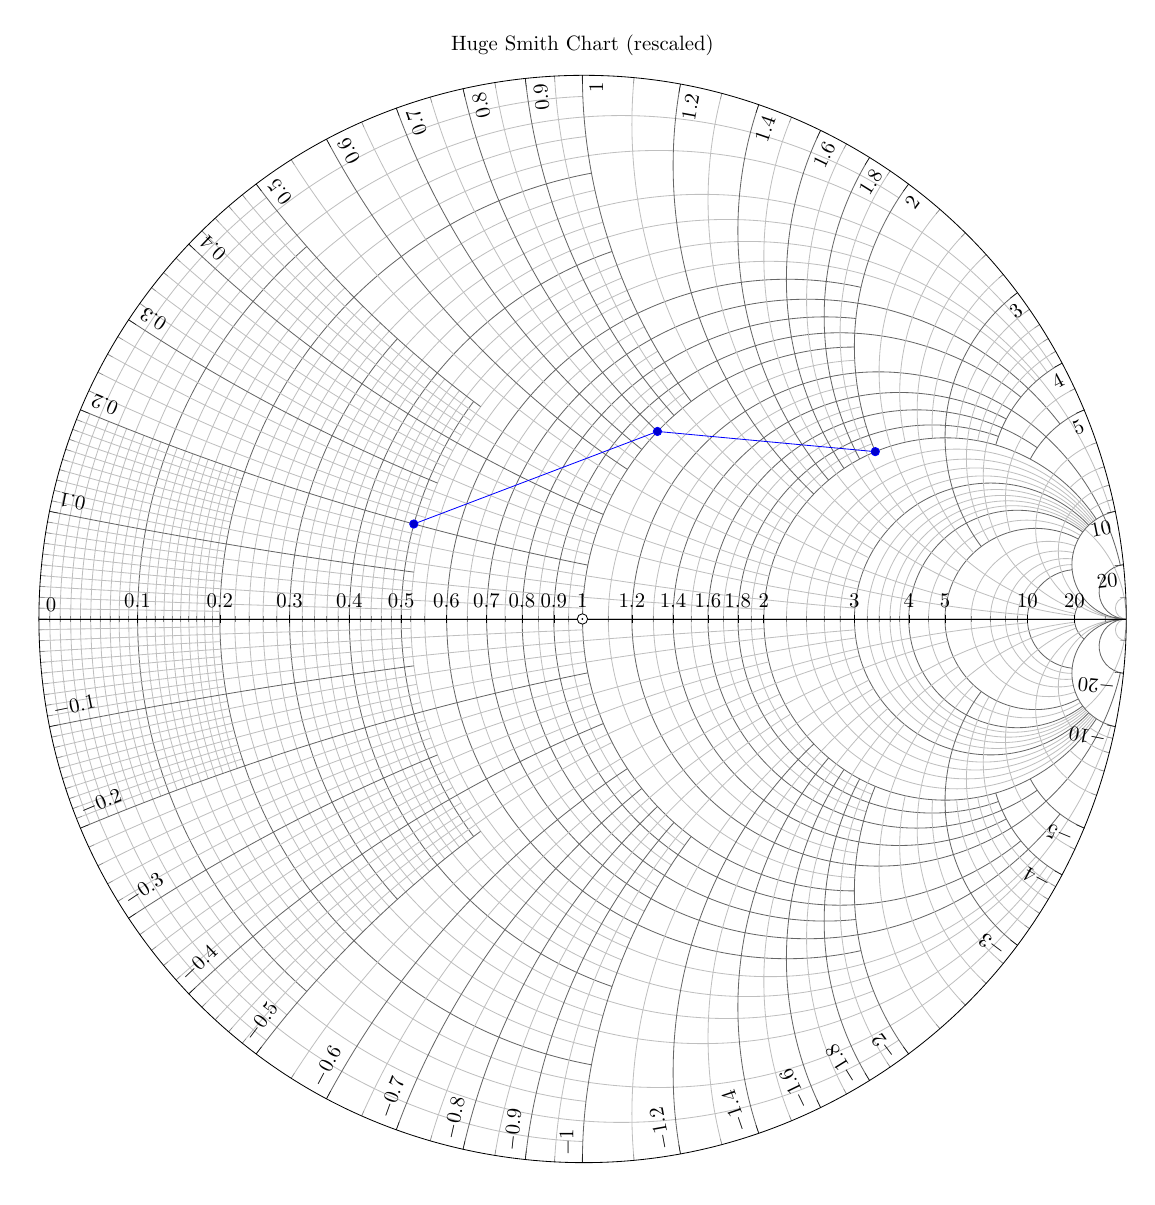
\begin{tikzpicture}[scale=0.75]
	\begin{smithchart}[
		title=Huge Smith Chart (rescaled),
		width=20cm]
	\addplot coordinates {(0.5,0.2) (1,0.8) (2,2)};
	\end{smithchart}
\end{tikzpicture}
\end{codeexample}

	\textbf{Attention:} This style might change in future versions!

	Similarly to |many smithchart ticks| (see above), the initial configuration is realized by means of \emph{two} separate styles: one which defines only the tick positions (the \declareandlabel{many smithchart ticks*} style) and one which also changes placement- and alignment options:
\begin{codeexample}[code only]
\pgfplotsset{
	dense smithchart ticks*/.style={
		default smithchart xtick/.style={
			xtick={
				0.1,0.2,0.3,0.4,0.5,0.6,0.7,0.8,0.9,1,1.2,1.4,1.6,1.8,2,3,4,5,10,20%
			},
			minor xtick={%
				0.01,0.02,0.03,0.04,0.05,0.06,0.07,0.08,0.09,0.11,0.12,0.13,0.14,0.15,0.16,0.17,
				0.18,0.19,0.22,0.24,0.26,0.28,0.32,0.34,0.36,0.38,0.42,0.44,0.46,0.48,%
				0.52,% This is sub-optimal and will (hopefully) be improved in the future.
				0.55,0.65,0.75,0.85,0.95,%
				%0.6,0.7,0.8,0.9,%
				1.1,1.3,1.5,1.7,1.9,%
				2.2,2.4,2.6,2.8,3.2,3.4,3.6,3.8,4.5,6,7,8,9,50},
		},
		default smithchart ytick/.style={
			ytick={%
				0,%
				0.1,0.2,...,1,1.2,1.4,1.6,1.8,2,3,4,5,10,20,%
				-0.1,-0.2,...,-1,-1.2,-1.4,-1.6,-1.8,-2,-3,-4,-5,-10,-20%
			},
			minor ytick={%
				0.01,0.02,0.03,0.04,0.05,0.06,0.07,0.08,0.09,0.11,0.12,0.13,0.14,0.15,0.16,0.17,
				0.18,0.19,0.22,0.24,0.26,0.28,0.32,0.34,0.36,0.38,0.42,0.44,0.46,0.48,%
				0.55,0.65,0.75,0.85,0.95,%
				1.1,1.3,1.5,1.7,1.9,2.2,2.4,2.6,2.8,3.2,3.4,3.6,3.8,4.5,6,7,8,9,50,%
				-0.01,-0.02,-0.03,-0.04,-0.05,-0.06,-0.07,-0.08,-0.09,-0.11,-0.12,-0.13,-0.14,
				-0.15,-0.16,-0.17,-0.18,-0.19,-0.22,-0.24,-0.26,-0.28,-0.32,-0.34,-0.36,-0.38,
				-0.42,-0.44,-0.46,-0.48,-0.55,-0.65,-0.75,-0.85,-0.95,%
				-1.1,-1.3,-1.5,-1.7,-1.9,-2.2,-2.4,-2.6,-2.8,-3.2,-3.4,-3.6,-3.8,-4.5,-6,-7,-8,
				-9,-50%
			},
		},
		default smithchart xytick/.style={
			xgrid each nth passes y={0.2 if < 0.2001,0.5 if < 0.50001,1 if < 1.001,2,4,5,10,20},
			ygrid each nth passes x={0.2 if < 0.2001,0.52 if < 0.52001,1 if < 1.001,2,3,5,10:3,20:3},
		},
	},
	dense smithchart ticks/.style={
		yticklabel in circle,
		dense smithchart ticks*,
		show origin=true,
		every major grid/.style={black!60},
	},
}
\end{codeexample}
	\noindent See the documentation for |few smithchart ticks| for an explanation of the |default smithchart xtick/.style| overhead.
\end{stylekey}

\begin{pgfplotskeylist}{%
	default smithchart xtick,%
	default smithchart ytick,%
	default smithchart xytick}
	The |default smithchart xtick| style is installed if and only if you do not provide |xtick| manually.

	Similarly, the |default smithchart ytick| style is installed if and only if you do not provide |ytick| manually.

	Finally, the |default smithchart xytick| style is installed if and only if you provide neither |xtick| nor |ytick|.

	These styles are usually defined in |few smithchart ticks| and its variants, see above.
\end{pgfplotskeylist}

\subsubsection{Working with Prepared Data}
\begin{pgfplotskey}{is smithchart cs=\mchoice{true,false} (initially false)}
	Occasionally, you may already have input data transformed into unit--circle Cartesian coordinate $r(z) = (x,y)$.

	You can provide them to \PGFPlots\ with the |is smithchart cs| key:
\begin{codeexample}[]
\begin{tikzpicture}
	\begin{smithchart}
	% smithchart_data.dat contains 
	% 0.78395 -0.40845
	% 0.78165 -0.41147
	% 0.77934 -0.41466
	% 0.77774 -0.41869
	% ...
	\addplot[blue,is smithchart cs] 
	  file {plotdata/smithchart_data.dat};
	\end{smithchart}
\end{tikzpicture}
\end{codeexample}
	Using |is smithchart cs| tells \PGFPlots\ to skip the transformation $r(z)$.
\end{pgfplotskey}

\subsubsection{Appearance Control and Styles}
\begin{pgfplotskey}{show origin=\mchoice{true,false} (initially false)}
	Allows to place an extra description at the point $(0,0)$ to mark the origin.
\begin{codeexample}[]
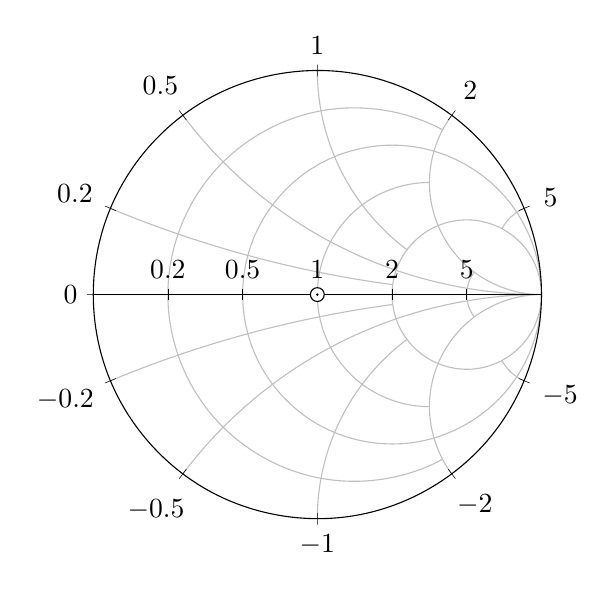
\begin{tikzpicture}
	\begin{smithchart}[show origin]
	\end{smithchart}
\end{tikzpicture}
\end{codeexample}
\begin{pgfplotscodekey}{show origin code}
	Allows to redefine the code to draw the origin marker. The initial configuration is
\begin{codeexample}[code only]
\pgfplotsset{
	show origin code/.code={%
		\path[draw=black,fill=white] (0pt,0pt) circle (2.5pt);
		\path[fill=black] (0pt,0pt) circle (0.5pt);
	}
}
\end{codeexample}
\end{pgfplotscodekey}
\end{pgfplotskey}

\begin{stylekey}{/pgfplots/yticklabel in circle}
	This style draws Smith Chart tick labels for imaginary components (the |ytick| arguments) inside of the circle.

	It installs transformations to rotate and shift tick labels. See the |many smithchart ticks| style for an example.

	The initial configuration for this style is
\begin{codeexample}[code only]
\pgfplotsset{
	yticklabel in circle/.style={
		ytick align=inside,
		yticklabel style={
			rotate=90,
			sloped like y axis={%
				execute for upside down={\tikzset{anchor=north east}},
				%allow upside down,
				reset nontranslations=false},
			anchor=south west,
			%font=\tiny,
		}
	}
}
\end{codeexample}
\end{stylekey}

\begin{stylekey}{/pgfplots/every smithchart axis}
	This style is installed for every Smith Chart. It is defined as
\begin{codeexample}[code only]
\pgfplotsset{
	every smithchart axis/.style={
		grid=both,
		xmin=0,
		scaled ticks=false, % never draw the \cdot 10^4 labels
		major tick style={draw=black},
		xtick align=center,
		ytick align=center,
	},
}
\end{codeexample}
\end{stylekey}

\subsubsection{Controlling Arcs and Their Stop Points}
This section allows advanced control over Smith Chart arcs (grid lines). The two features |xgrid each nth passes y| and |xgrid stop at y| (and their counterparts for $y$) allow to draw only partial arcs in order to get a more uniform appearance.

\begin{pgfplotskey}{xgrid each nth passes y=\marg{list of stop entries} (initially empty)}
	This key constitutes the main idea to draw only partial arcs: you provide a couple of $y$ tick coordinates which constitute ``boundaries''. Then, only each (say) second $x$ grid line is allowed to pass these boundaries:
\begin{codeexample}[]
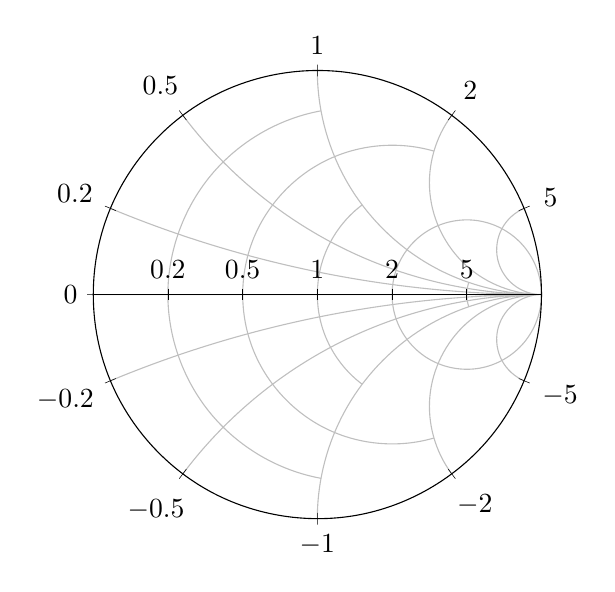
\begin{tikzpicture}
	\begin{smithchart}[
		xtick={0.2,0.5,1,2,5},
		ytick={
			0,
			 0.2, 0.5, 1, 2, 5,
			-0.2,-0.5,-1,-2,-5},
		xgrid each nth passes y={1,2},
	]
	\end{smithchart}
\end{tikzpicture}
\end{codeexample}
	The example overwrites the |default smithchart ticks| to define a new layout: now, every |ytick| uses the complete arc, but some of the grid lines for |xtick| stop at $y=1$ and, if they pass, they may stop at $y=2$.

	The argument \meta{list of stop entries} is a comma--separated list of entries. Each entry is, in the simplest case, a $y$ coordinate (it should be a coordinate which appears in the |ytick| list). This simplest case means ``only each second $x$ grid line may pass the grid line for this $y$''. The second syntax allows to provide a natural number, using \meta{y coord}|:|\meta{number}. This means to let only each \meta{number}'s $x$ grid line pass the designated $y$ grid line. The third syntax also allows to write |if < |\meta{x value}. It means the entry is considered only for $x$ grid lines which are less than \meta{x value}. To summarize: there are the three possible forms of entries
	\begin{enumerate}
		\item single $y$ coordinates, for example |xgrid each nth passes y={1,2}| or
		\item the same as above, followed by an integer, for example |xgrid each nth passes y={1:3,2:2}| or
		\item an additional restriction clause like |xgrid each nth passes y={0.2 if <0.3}|. 
		
		In this case, the all $x$ grid lines which fulfill $x \le 0.3$ will be checked if they are allowed to pass $y=0.2$. All $x$ grid lines with $x > 0.3$ are not affected by the constraint. See the |dense smithchart ticks| style for an application example.
	\end{enumerate}

	Note that |xgrid each nth passes y| always employs symmetry; you do not need to provide $y$ and $-y$ (if you want to, you may use the |xgrid stop at y| key to overrule the ``each nth''-strategy).


	In order to check if a given |xtick| argument is the ``$n$th'' grid line, \PGFPlots\ collects all |xtick| and |minor xtick| arguments into \emph{one} large array and sorts it. Then, it uses the resulting sequence to assign the indices. Consequently, you can freely intermix minor and major ticks; it will still work. The only way to affect the counting is the |xgrid each nth passes y start| key, see below.
\end{pgfplotskey}

\begin{pgfplotskey}{ygrid each nth passes x=\marg{list of stop entries} (initially empty)}
	As you may already have guessed, this is the $y$ counterpart of |xgrid each nth passes y|. It restricts the arcs for $y$ grid lines by provided $x$ ticks:
\begin{codeexample}[]
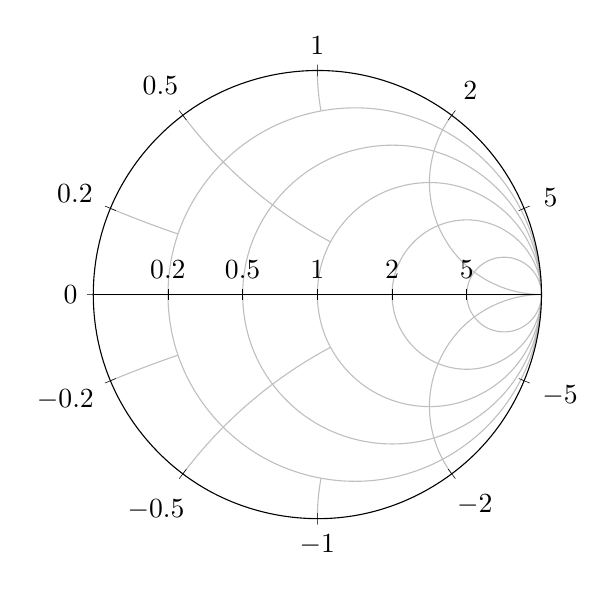
\begin{tikzpicture}
	\begin{smithchart}[
		xtick={0.2,0.5,1,2,5},
		ytick={
			0,
			 0.2, 0.5, 1, 2, 5,
			-0.2,-0.5,-1,-2,-5},
		ygrid each nth passes x={0.2,1:2},
	]
	\end{smithchart}
\end{tikzpicture}
\end{codeexample}
	The syntax is exactly the same as explained for |xgrid each nth passes y|. The only difference is that the |if <| syntax uses absolute values $|y|$ (to maintain symmetry).
\end{pgfplotskey}

Now, we know how to use |xgrid each nth passes y| and the corresponding |ygrid each nth passes x| \emph{separately}. Can we use both keys at the same time? Yes -- but it may happen that lines end in white space! \PGFPlots\ applies some logic to avoid arcs ending in white space by extending them to the next feasible stopping point. The result of mixing both of these keys is thus corrected automatically.

\begin{pgfplotskeylist}{%
	xgrid each nth passes y start=\marg{integer} (initially 0),%
	ygrid each nth passes x start=\marg{integer} (initially 0)}
	Allows to modify where the ``each $n$th'' counting starts. The argument can be considered as a shift. I consider this key to be more or less experimental -- in the hope it may be useful. Try it out.
\end{pgfplotskeylist}

\begin{pgfplotskeylist}{%
	xgrid stop at y=\marg{list} (initially empty),
	ygrid stop at x=\marg{list} (initially empty)}
	These keys allow to provide \emph{individual} stop points for explicitly chosen tick positions. These explicit stop points have higher precedence over the each nth features described above.

	The |ygrid stop at x| key accepts a comma--separated list of entries \meta{y coord}|:|\meta{x stop point}:
\begin{codeexample}[]
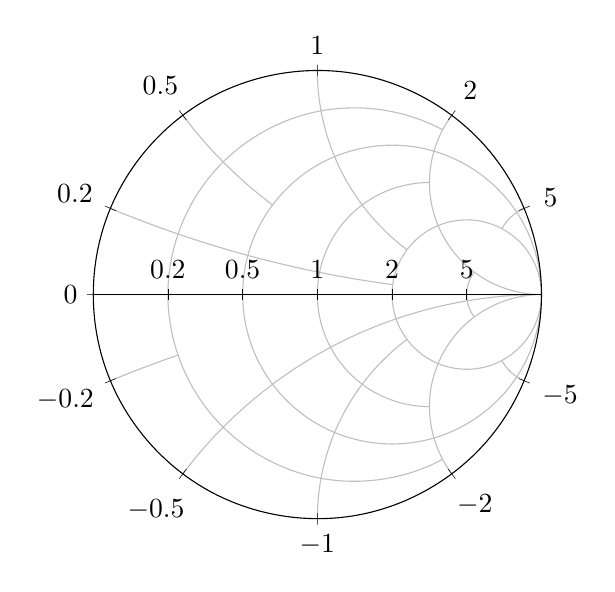
\begin{tikzpicture}
	\begin{smithchart}[
		ygrid stop at x={0.5:0.5,-0.2:0.2}
	]
	\end{smithchart}
\end{tikzpicture}
\end{codeexample}
	\noindent In this example, the $y=0.5$ arc stops at the $x=0.5$ arc whereas the $y=-0.2$ arc stops at $x=0.2$.

	The |ygrid stop at x| key allows unsymmetric layouts (different stop points for $y$ and $-y$).
\end{pgfplotskeylist}


\end{document}

